\documentclass[11pt]{article}

% ==========================================================================
% chi-VLA: Fully Tensor-Decomposable Vision-Language-Action Models
% Compile: pdflatex chi-vla.tex  (twice, for references)
% ==========================================================================

\usepackage[margin=1in]{geometry}
\usepackage{amsmath,amssymb,amsfonts}
\usepackage{booktabs}
\usepackage{graphicx}
\usepackage{xcolor}
\usepackage{tikz}
\usetikzlibrary{positioning,fit,backgrounds,arrows.meta}
\usepackage[colorlinks=true,linkcolor=blue,citecolor=blue,urlcolor=blue]{hyperref}
\usepackage{caption}
\usepackage{float}

\newcommand{\chivla}{$\chi$-VLA}
\newcommand{\chivit}{$\chi$-ViT}

\title{\textbf{Convertibility Is Nearly Free:}\\[0.2em]
\textbf{A Capable, Fully Tensor-Decomposable Vision-Language-Action Model}\\[0.4em]
\large Convertibility is nearly free for language models, but not automatically for
multimodal ones. We recover it: multimodal action decoding and rational per-instance
normalization within the (rational) tensor-network class, with weight-based interpretability
for free}
\author{}
\date{\today}

\begin{document}
\maketitle

\begin{abstract}
A line of work replaces every nonlinearity in a network with bilinear/polynomial
operations, so the whole learned map is a single tensor network that can be decomposed, and interpreted, directly from its weights. The unspoken price is \emph{capability}: the
operations a capable policy needs but a polynomial cannot express, multimodal action
decoding, per-instance normalization, seem to force a softmax, a sampler, or an
input-dependent division that leaves the tensor-network class. This tax was already shown to
be small for \emph{language} models, whose sole output nonlinearity is a categorical softmax
that lives outside the learned map as a decode, but it does \emph{not} transfer automatically
to multimodal policies, whose output is a continuous, jointly multimodal action distribution
rather than a categorical next-token pick. We show the tax is nonetheless largely recoverable,
and build \chivla, a Vision-Language-Action policy (pixels $+$ instruction $\to$ robot actions)
whose learned blocks admit a fully tensor-decomposable polynomial or rational configuration.
\textbf{(1) Multimodal control without leaving the tensor network.} If the learned action
\emph{distribution} is kept in-graph and polynomial and only the \emph{decode} is moved
outside (a routing sign, exactly the status of OpenVLA's external argmax), a genuinely
multimodal action head can be built \emph{only} from CP cores, addressing the fact that a
linear-mean head is an invalid ``average of valid behaviours'' wherever the demonstrations
are multimodal ($\sim$$40\%$ of states, which we measure). Such a head drives non-trivial
end-to-end closed-loop control in the LIBERO-Object simulator. At our small, from-scratch
scale we make \emph{no} claim that the multimodal head outperforms the linear-mean head
because their seed ranges overlap under matched evaluation. The contribution is
representational, that a multimodal action distribution can be carried and controlled
entirely in-graph. \textbf{(2) Per-instance normalization in the rational tensor-network
class.} Mean-square normalization folds \emph{exactly} in projective (numerator,
denominator) coordinates into a ratio $P(x)/Q(x)$ of polynomial tensor networks, verified
to $10^{-14}$. A fixed rational approximation to inverse square root gives an RMS-like
per-token operator within the same rational class. Together (1)--(2) recede both inherently-nonlinear costs
behind one principle: \emph{keep the learned object in-graph and polynomial/rational. Decode
outside.} \textbf{(3) Interpretability comes for free, coherence is bought by topology.}
The exact weight-derived orthogonalize--diagonalize--truncate (ODT) basis is causally faithful
(matching PCA and integrated gradients, far exceeding random on deletion/insertion) and
survives attention. Whether its atoms are \emph{human-coherent} is set by topology, not
convertibility (spatial-locality-preserving models reach $\sim$$3.5\times$ random-baseline
locality), confirming and, with interventions, matched capability, and a policy
bond-placement principle, extending prior bilinear-interpretability work. Honest scope: the
interpretability payoff is a causal, rankable, topology-tunable basis and a locality
\emph{metric}, not yet a gallery of nameable features. Our strongest closed-loop checkpoint
reaches $94.2\%\pm1.2\%$ on eight of ten LIBERO-Object tasks, using a $600$-step cap and
per-token RMS normalization, its one remaining non-foldable operator. Replacing that operator
with the rational per-instance norm and retraining from scratch makes every learned site a
polynomial or rational tensor primitive by construction. This model reaches
$\mathbf{94.5\%}$ ($189/200$) on all ten LIBERO-Object tasks in one seed. No capability loss
is visible in this point estimate, although the per-token and rational evaluations differ in
suite coverage and seed count. The OpenVLA study reports $88.4\%\pm0.8\%$ for OpenVLA and
$92.5\%\pm0.7\%$ for Diffusion Policy over all ten tasks with a $280$-step cap
\cite{openvla}. Our evaluation uses a looser $600$-step cap and fewer trials, so we make no
state-of-the-art claim. We further verify decomposability on the trained checkpoint itself, not
just architecturally: a mechanical audit confirms every module the policy actually invokes is
polynomial or rational with zero exceptions, and an exact projective fold-and-verify on the real
trained weights reproduces the deployed computation to the float32 precision floor
(\S\ref{subsec:decompaudit}). A real causal intervention in the live simulator (swapping which
co-present object the instruction names) gives an honest negative (switch-rate $15.6\%$,
\S\ref{subsec:realintervention}), which we attribute to real training data confounding scene
identity with instruction, a limitation the synthetic-task intervention was built to avoid. The
result establishes the narrower claim that rational tensor construction is compatible with
competitive closed-loop control.
\end{abstract}

\begin{figure}[h]
\centering
\begin{minipage}[t]{0.53\textwidth}
\centering
\resizebox{\linewidth}{!}{%
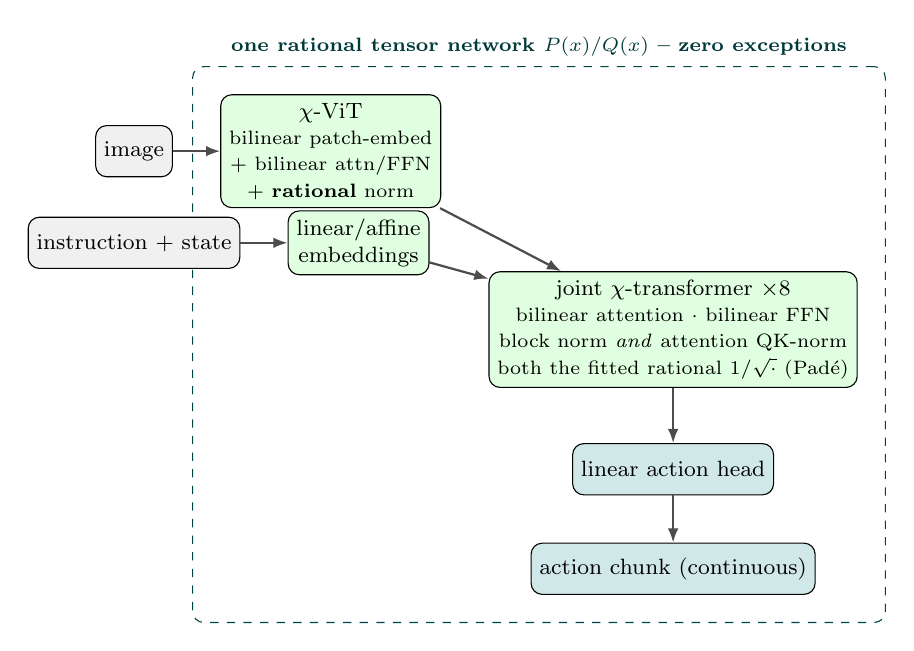
\begin{tikzpicture}[
  font=\footnotesize,
  box/.style={draw, rounded corners, align=center, minimum height=6.5mm, inner sep=3pt},
  inp/.style={box, fill=gray!12},
  prim/.style={box, fill=green!12},
  outbox/.style={box, fill=teal!18},
  arr/.style={-{Latex[length=1.8mm]}, thick, gray!60!black},
  node distance=5mm and 6mm,
]
\node[inp] (img) {image};
\node[inp, below=of img] (lang) {instruction $+$ state};
\node[prim, right=of img] (vit) {$\chi$-ViT\\{\scriptsize bilinear patch-embed}\\{\scriptsize $+$ bilinear attn/FFN}\\{\scriptsize $+$ \textbf{rational} norm}};
\node[prim, right=of lang, minimum height=6.5mm] (emb) {linear/affine\\embeddings};
\node[prim, below right=8mm and 6mm of vit, minimum width=30mm] (bb) {joint $\chi$-transformer $\times 8$\\{\scriptsize bilinear attention $\cdot$ bilinear FFN}\\{\scriptsize block norm \emph{and} attention QK-norm}\\{\scriptsize both the fitted rational $1/\sqrt{\cdot}$ (Pad\'e)}};
\node[outbox, below=7mm of bb] (head) {linear action head};
\node[outbox, below=6mm of head] (act) {action chunk (continuous)};
\draw[arr] (img) -- (vit); \draw[arr] (lang) -- (emb);
\draw[arr] (vit) -- (bb); \draw[arr] (emb) -- (bb);
\draw[arr] (bb) -- (head); \draw[arr] (head) -- (act);
\begin{scope}[on background layer]
\node[draw=teal!55!black, dashed, rounded corners, fit=(vit)(emb)(bb)(head)(act),
      inner sep=3.5mm, label={[teal!45!black,font=\scriptsize\bfseries]above:one rational tensor network $P(x)/Q(x)$ -- zero exceptions}] {};
\end{scope}
\end{tikzpicture}}
\end{minipage}%
\hfill
\begin{minipage}[t]{0.44\textwidth}
\centering
\small
\begin{tabular}{@{}lcc@{}}
\toprule
\textbf{Model} & \textbf{Tasks} & \textbf{Success} \\
\midrule
\chivla, rational norm & $10/10$ & $\mathbf{94.5\%}$ \\
\chivla, per-token norm & $8/10$ & $94.2\%\pm1.2\%$ \\
\chivla, conv vision & $8/10$ & $90.8\%\pm0.3\%$ \\
\midrule
Diffusion Policy \cite{openvla} & $10/10$ & $92.5\%\pm0.7\%$ \\
OpenVLA-7B \cite{openvla} & $10/10$ & $88.4\%\pm0.8\%$ \\
\bottomrule
\end{tabular}
\vspace{2mm}

\raggedright\scriptsize Closed-loop success, LIBERO-Object. Settings differ (step cap,
trials/task, seeds -- Table~\ref{tab:closedloop-comparison}); not a matched
state-of-the-art claim. \chivla\ is $\sim$$20$M parameters, trained from scratch,
no pretraining.
\end{minipage}
\caption{\textbf{The current fully-tensor \chivla\ (left) and its best closed-loop results
(right).} With a plain linear head, every learned computation -- vision, joint attention
backbone, normalization, and the action output itself -- is one polynomial/rational tensor
network; there is no out-of-graph decode step at all in this configuration (contrast the
multimodal head, Fig.~\ref{fig:head}, whose sign-routing decode is the one exception).}
\label{fig:at-a-glance}
\end{figure}

% ============================================================================
\section{Introduction}
% ============================================================================

Interpreting a large policy is hard largely because the network is not
compositional. Nonlinear operations such as the softmax in attention, the smooth
activation in an MLP, and layer normalization prevent us from rewriting the model
as a single algebraic formula, so we are forced to study its behaviour on data
rather than its weights directly. A recent line of work argues that this is a
design choice, not a necessity. If every learned operation is kept polynomial in
the activations, built only from linear maps, element-wise multiplications,
additions, fixed masks and permutations, learned constants, and fixed scalar or
diagonal rescalings, then the whole model is a single multilinear object, a
\emph{tensor network}, that can be decomposed, ranked, and truncated using
numerical linear algebra applied to the weights alone, no data required. The
three subsections below state, in order, the question we ask, the prior results
we build directly on, and what in this paper is new.

\subsection{Goal}

\emph{What does full tensor-decomposability actually cost a capable policy, and what
does it buy?} The standing worry is that forcing every operation to be polynomial
trades away real capability for the promise of interpretability. This is an open
question specifically for \emph{vision-language-action} (VLA) policies, whose output is a
continuous, jointly multimodal action distribution rather than a language model's
categorical next-token pick, and whose normalization sits inside a
perception-heavy, degree-two-amplifying stack. We build \chivla, a VLA policy
(pixels $+$ instruction $\to$ robot actions) whose learned blocks admit a fully
tensor-decomposable polynomial or rational configuration, and use it to answer the
question directly: train it, close the loop in a real simulator, and interrogate
its weights.

\subsection{What this builds on}

Convertibility, i.e.\ replacing every nonlinearity with a polynomial or bilinear
primitive, was already shown to be nearly free for two narrower settings, and we
assemble both into one policy.

\paragraph{Convertibility is nearly free for language models \cite{riggs,chinets}.} A
language model's only output nonlinearity is the categorical softmax, and that softmax is
a \emph{decode}: linear logits go in, an $\arg\max$ or a sample comes out, and the pick
already lives outside the learned map. Making the rest of the network polynomial therefore
costs almost nothing, because the one hard operation was never in the tensor network to
begin with. Riggs \cite{riggs} gives the two core primitives we reuse throughout, the
bilinear (CP-factorized) feed-forward layer and softmax-free bilinear attention. Dooms et
al.\ \cite{chinets} give foldable (frozen-scalar) normalization and
Orthogonalize--Diagonalize--Truncate (ODT), the procedure for exactly, globally
decomposing a tree-shaped tensor network, as a \emph{compression} result.

\paragraph{The policy skeleton: OpenVLA \cite{openvla}.} We keep the modular OpenVLA
pipeline (vision encoder(s) $\to$ projector $\to$ language-model backbone $\to$ action
decoder) and replace each of its four learned stages with the corresponding published
polynomial primitive:

\begin{itemize}
  \item \textbf{Bilinear feed-forward layer} (Riggs \cite{riggs}). Replace the
        gated MLP $D(\mathrm{swish}(Lx)\otimes Rx)$ with the activation-free
        $D[(L\bar x)\otimes(R\bar x)]$, where $\otimes$ is the element-wise
        (Hadamard) product and $\bar x$ is defined below. This is exactly a
        low-rank factorization (a CP, or canonical polyadic, factorization) of a
        third-order weight tensor.
  \item \textbf{Softmax-free bilinear attention} (Riggs \cite{riggs}). Replace the
        softmax attention pattern with the element-wise product of two separate
        learned query-key score matrices.
  \item \textbf{Foldable normalization} (Dooms et al. \cite{chinets}). Normalize
        during training by dividing by a running average magnitude (a single
        scalar), then after training freeze that scalar and multiply it into the
        next weight matrix, so the deployed model contains no division at all.
  \item \textbf{Linear action head}. Replace the discretized action tokens and
        language-model-style decoding with a direct linear map from learned
        action-query states to a continuous action vector.
\end{itemize}

We assemble these along the OpenVLA skeleton, keeping only genuinely non-learned
interfaces outside the tensor-network boundary (tokenization, camera decoding, safety
clipping, motor communication), so that \chivla's learned map from pixels and token
identities to a continuous action is, by construction, one tensor network.

\subsection{What is novel here}

Two of the four borrowed replacements above are \emph{not} actually solved by the
published primitives once the policy has to be capable, and the interpretability
literature they enable has, so far, never been run on a real, working, closed-loop
robot policy. Both gaps are what this paper adds.

\paragraph{Novelty 1: recovering the two operations that generically break convertibility.}
A linear action head trained by MSE can only emit a conditional \emph{mean}, which is an
invalid ``average of valid behaviours'' whenever demonstrations are multimodal ($\sim$$40\%$
of LIBERO-Object states, which we measure), and the frozen-scalar norm only
\emph{approximates} true per-instance normalization. Neither failure is addressed by prior
tensor-pure work, because neither arises for a language model. We show both are recoverable
\emph{within} the polynomial/rational tensor-network class, not by relaxing it: (i) a
multimodal action head built entirely from CP cores, whose learned \emph{distribution}
stays in-graph and only a routing \emph{sign} is decoded outside (the same status OpenVLA
gives its argmax); and (ii) per-instance normalization carried in projective
(numerator, denominator) coordinates, which folds \emph{exactly} into a ratio $P(x)/Q(x)$
of two polynomial tensor networks, verified to $10^{-14}$, with a fixed rational
approximation to $1/\sqrt{\cdot}$ giving an RMS-like operator in the same class. One
principle covers both: \emph{keep the learned object in-graph and polynomial/rational,
decode outside}.

\paragraph{Novelty 2: the interpretability payoff, measured on a real, competitive, closed-loop policy.} Prior tensor-interpretability work stops at compression (Dooms et al.
\cite{chinets}) or asserts, without an intervention, that architecture affects eigen-feature
coherence on shallow classifiers (Pearce et al.\ \cite{riggs}; D\'eh\'erand
\cite{deherand}). We instead (i) separate \emph{causal} from \emph{coherent} as an explicit,
intervention-tested axis with standard faithfulness baselines, (ii) establish topology, not
convertibility, as the coherence lever at matched capability, with depth-scaling and
cross-dataset de-risking, (iii) introduce a \emph{bond-placement} principle for policies (a
mechanism is decodable only at the bond downstream of the attention that constructs it), and
(iv) run all of this on \chivla's actual trained, closed-loop LIBERO-Object policy, not only
on classifiers or a synthetic task.

Our contributions, established across substrates of increasing difficulty (image
classifiers, a softmax-free vision transformer, the full tensor-decomposable policy, and its
closed-loop control), are:

\begin{enumerate}
  \item \textbf{Multimodal control without leaving the tensor network.} Keeping the learned
        action \emph{distribution} in-graph and polynomial and moving only the \emph{decode}
        outside, a genuinely multimodal action head can be built only from CP cores, since a
        linear-mean head is invalid wherever the demonstrations are multimodal ($\sim$$40\%$
        of states, measured). Such a head achieves non-trivial closed-loop success on the
        LIBERO-Object simulator. At our small, from-scratch scale the product and linear
        head seed ranges overlap, so we make no superiority claim. The contribution is that
        a multimodal action distribution is representable and controllable entirely in-graph.
  \item \textbf{Per-instance normalization in the rational tensor-network class.} Carried in
        projective (numerator, denominator) coordinates, mean-square normalization folds
        \emph{exactly} into $P(x)/Q(x)$ (both polynomial/CP), verified to $10^{-14}$. A fixed
        rational inverse-square-root approximation gives an RMS-like operator without a
        frozen scalar. Contributions 1--2 recede both inherently
        nonlinear costs behind one principle: \emph{learned object in-graph. Decode outside}.
  \item \textbf{Interpretability is free. Coherence is bought by topology.} The exact
        weight-derived ODT basis is causally faithful by deletion/insertion (matching PCA and
        integrated gradients, far exceeding random) and survives attention. Whether its atoms
        are human-coherent is set by topology, not convertibility (spatial-locality-preserving
        topology reaches $\sim$$3.5\times$ random-baseline locality, at no accuracy cost). We
        add interventions, matched-capability controls, and depth-scaling to prior bilinear
        interpretability, and are honest that this coherence is a \emph{metric}, not yet a
        gallery of nameable features.
  \item \textbf{For a policy, mechanisms live behind the attention.} The action-relevant
        quantity is constructed by attention and readable only at a post-attention bond, and
        decoding it there is not the same as controlling it.
\end{enumerate}

Recovering novelty 1 (contributions 1--2), and closing the loop in simulation, is where the
architecture stops being a mere substrate and becomes part of the contribution; novelty 2
(contributions 3--4) is the interpretability payoff that substrate is built to support.

% ============================================================================
\section{Background: the three polynomial primitives}
% ============================================================================

\paragraph{The homogeneous coordinate.} Throughout, we write $\bar x = [1;x]$ for
the input with a constant $1$ prepended. This ``homogeneous coordinate'' lets a
bilinear layer represent not only quadratic terms but also linear terms and
constants (a bias becomes the weight on the constant coordinate). Without it, a
stack of $L$ multiplicative layers would be forced to produce only degree-$2^L$
terms. With it, the network can represent every degree up to $2^L$, including the
near-linear functions that most of a real task needs.

\paragraph{Bilinear feed-forward layer (a CP-factorized cubic tensor).} With
$L,R\in\mathbb{R}^{r\times(d+1)}$ and $D\in\mathbb{R}^{d\times r}$,
\begin{equation}
\mathrm{BFFN}(x) = D\big[(L\bar x)\otimes(R\bar x)\big],
\qquad
y_o = \sum_{i,j}\Big(\underbrace{\textstyle\sum_r D_{or}L_{ri}R_{rj}}_{T_{oij}}\Big)\bar x_i \bar x_j .
\end{equation}
The middle expression makes the tensor structure explicit: the layer is exactly a
third-order weight tensor $T\in\mathbb{R}^{d\times(d+1)\times(d+1)}$ contracted
twice with the input. The factored form uses about $3dr$ parameters instead of the
$d^3$ of the dense tensor, which is why it is called a CP factorization (a sum of
$r$ rank-one terms).

\paragraph{Softmax-free bilinear attention.} Each head forms two query-key systems
$A_1=Q_1K_1^\top$ and $A_2=Q_2K_2^\top$ and one value matrix $V$. The attention
pattern is their element-wise product, with no softmax:
\begin{equation}
Y = C\big[M \otimes (A_1\otimes A_2)/s\big]V .
\end{equation}
Here $M$ is a fixed mask (for example, lower-triangular for causal models), $C$ is
a fixed per-row rescaling $C_{ii}=1/\sqrt{n_i}$ with $n_i$ the number of visible
keys, and $s$ is a fixed scale. Because there is no softmax, the whole operation
is polynomial in the activations. It can be evaluated three mathematically
identical ways: the explicit $N\times N$ pattern. A ``Khatri-Rao'' form that
avoids the $N\times N$ matrix by building row-wise Kronecker features, and a
causal prefix-scan. We verified all three agree to $10^{-5}$ in single precision.

\paragraph{Foldable normalization.} During training we divide activations by a
single running scalar equal to their average root-mean-square magnitude. After
training we re-estimate that scalar on a calibration set, freeze it, and multiply
it into the following weight matrix ($W' = W/c$ before a linear map, or
$L'=L/c,\,R'=R/c$ before a bilinear layer). A frozen scalar division is a fixed
rescaling, so the deployed model has no operation whose divisor depends on the
input. This is what we mean by ``fold'': the normalization module disappears into
the weights.

% ============================================================================
\section{From OpenVLA to $\chi$-VLA}
% ============================================================================

Figure~\ref{fig:arch} contrasts the two pipelines and Table~\ref{tab:swaps} lists
the block-level replacements. The high-level flow is deliberately preserved, while
every learned internal block is replaced by a polynomial one.

\begin{figure}[t]
\centering
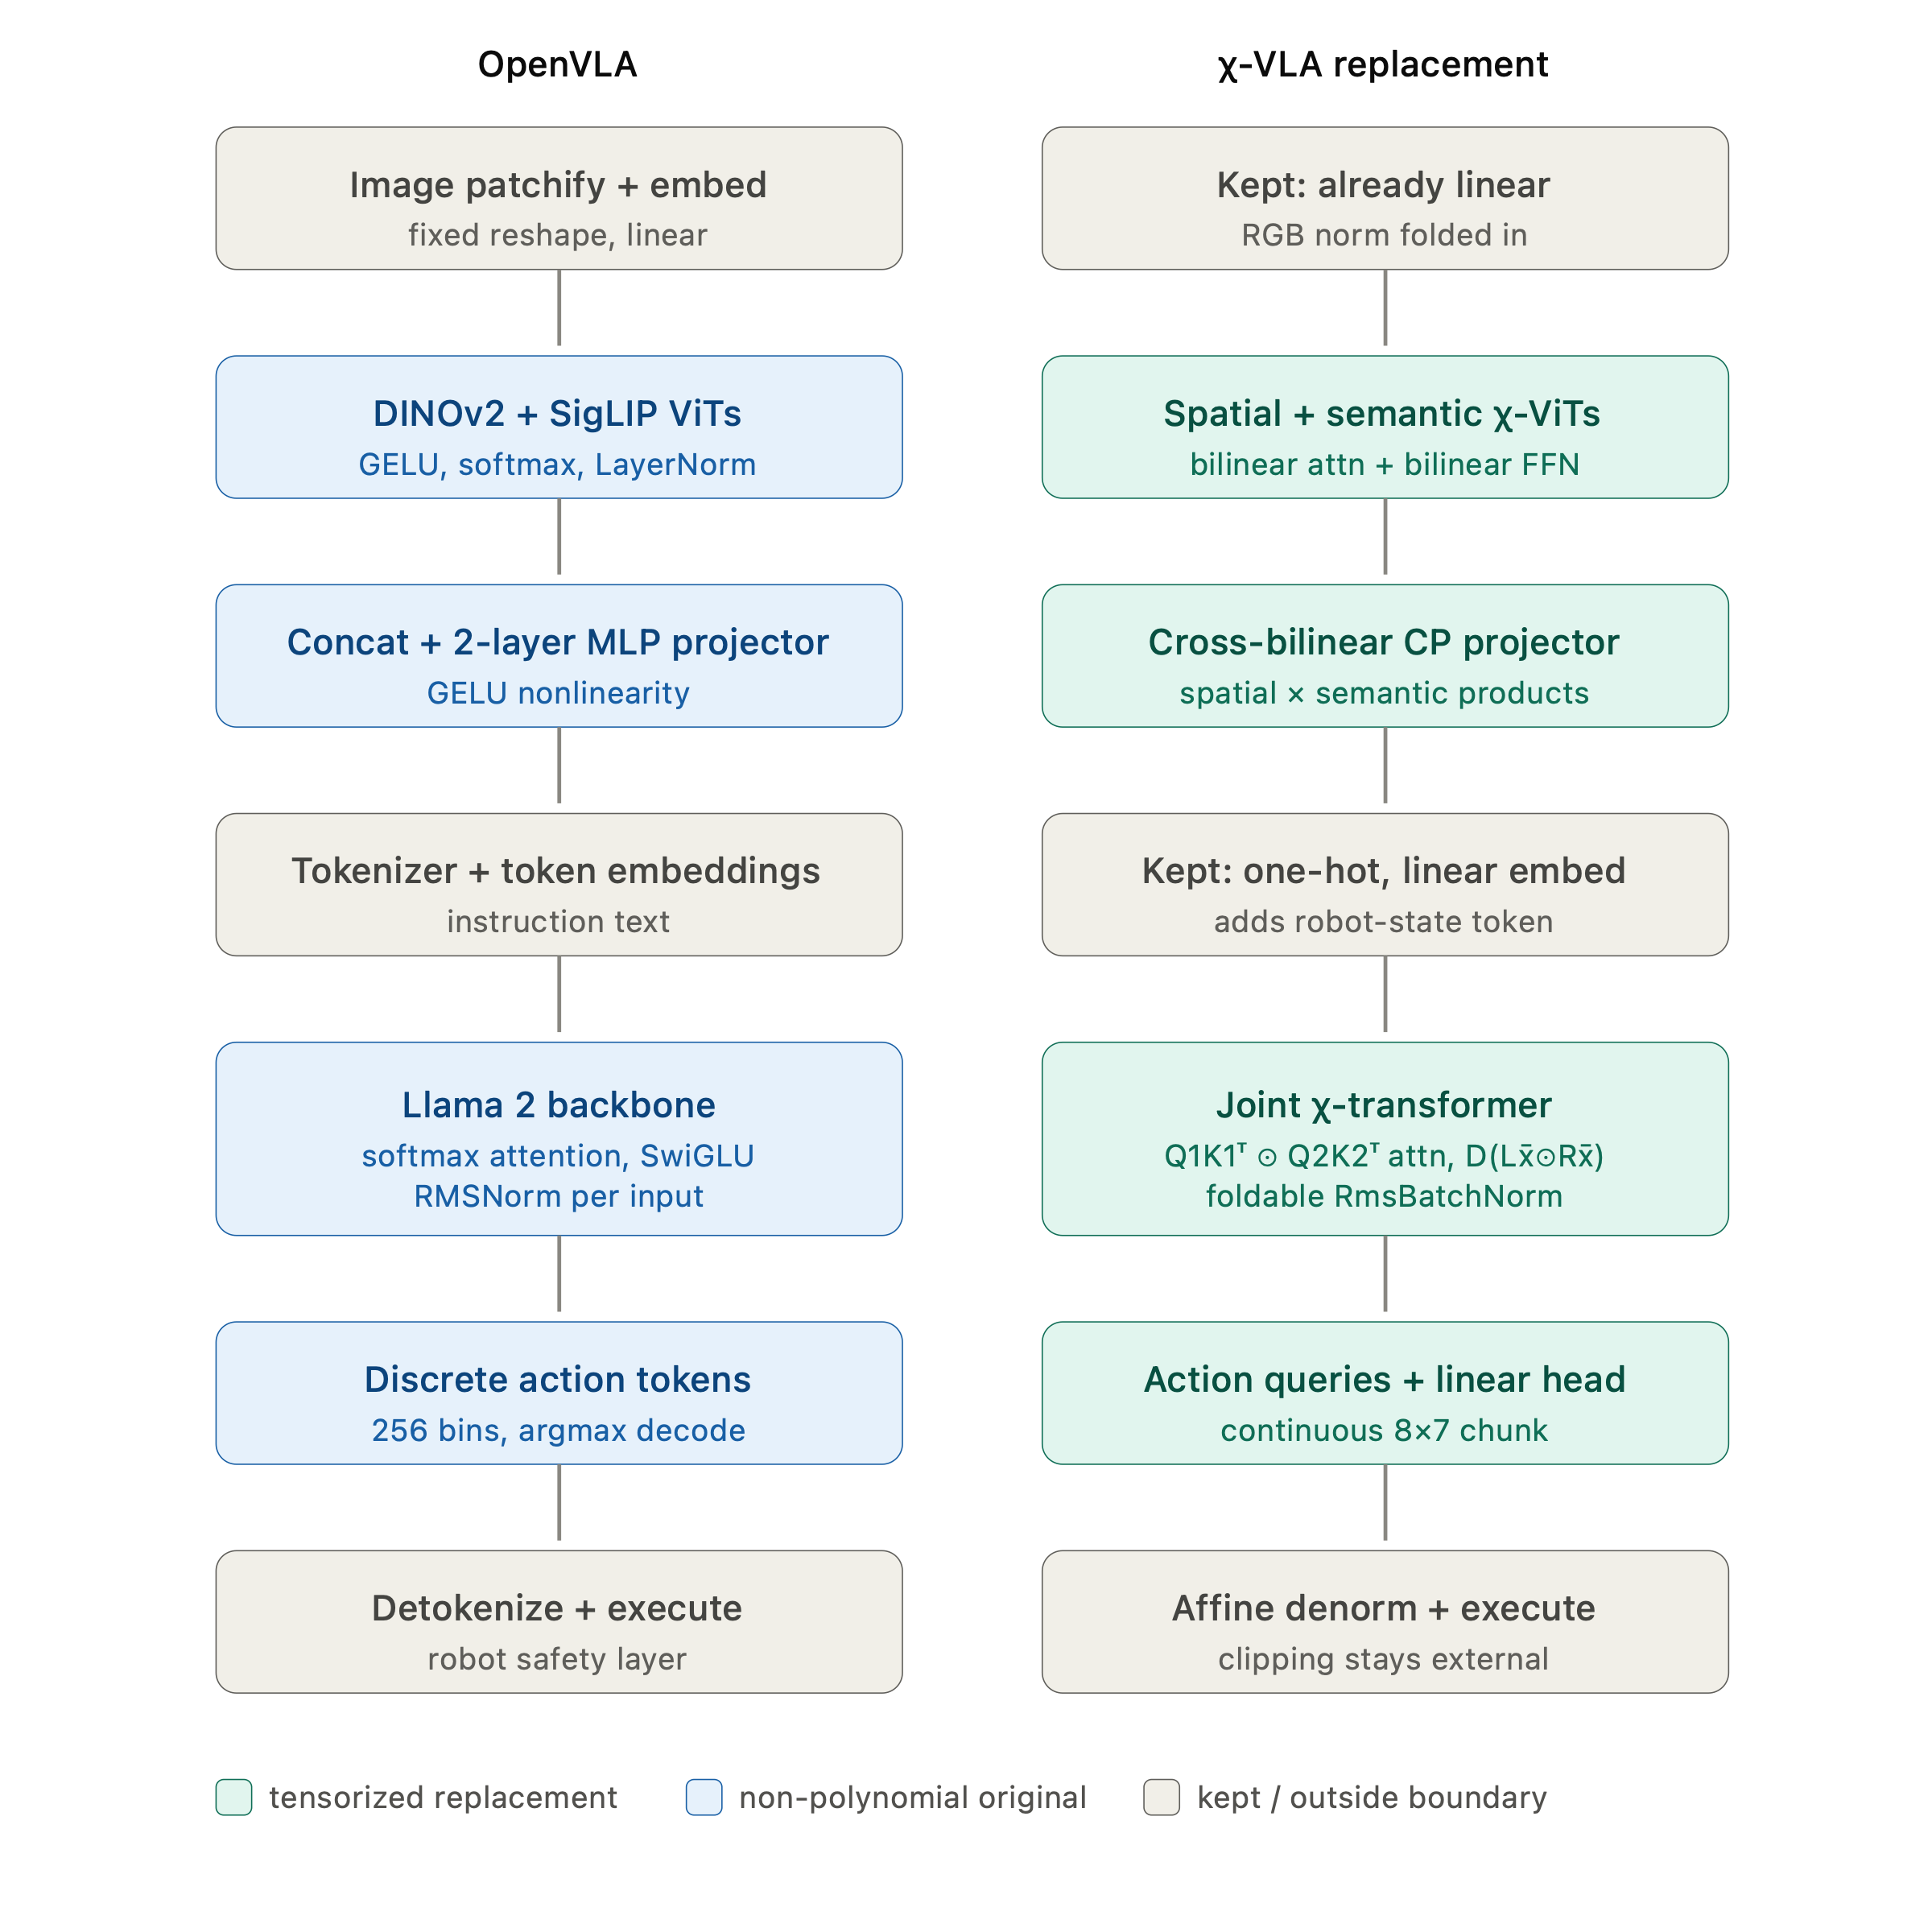
\includegraphics[width=0.84\textwidth]{pipeline.png}
\caption{OpenVLA (left) versus \chivla\ (right), stage by stage. Green boxes are
the polynomial (tensorized) replacements. Blue boxes are the non-polynomial
originals they replace. Grey boxes are kept unchanged or lie outside the
tensor-network boundary. Patch embedding and the tokenizer are already linear and
need no change. The softmax, smooth-activation, and layer-normalization blocks
(the dual vision encoders, the MLP projector, and the Llama~2 backbone) and the
discrete action decoder are each swapped for a polynomial equivalent with foldable
normalization. Camera decoding, string tokenization, and safety clipping stay
external.}
\label{fig:arch}
\end{figure}

\begin{table}[t]
\centering
\small
\resizebox{\textwidth}{!}{%
\begin{tabular}{@{}lll@{}}
\toprule
\textbf{Ordinary component} & \textbf{\chivla\ replacement} & \textbf{Algebraic form} \\
\midrule
Smooth activation (ReLU, GELU) & element-wise product of two linear maps & $(Lx)\otimes(Rx)$ \\
Gated MLP & bilinear (CP) feed-forward & $D[(L\bar x)\otimes(R\bar x)]$ \\
Softmax attention & product of two score matrices & $C[M\otimes(A_1\otimes A_2)/s]V$ \\
Layer/RMS normalization & foldable scalar \emph{or} rational per-instance norm & $x/c$ (frozen scalar) \emph{or} $P(x)/Q(x)$ (rational, exact) \\
MLP projector & cross-bilinear (CP) projector & $W_s s{+}W_m m{+}D_p[(L_s\bar s)\otimes(R_m\bar m)]$ \\
DINOv2 / SigLIP encoders & two polynomial \chivit s & (all blocks bilinear) \\
Llama~2 backbone & polynomial transformer & (all blocks bilinear) \\
Discrete action tokens (unimodal) & linear continuous-action head & $\hat a_k = W_a h_k + b_a$ \\
Discrete action tokens (multimodal) & product-routing mixture (CP cores) & $a = c_0(h){+}\sum_g \mathrm{sign}(g_g(h))\,c_g(h)$ \\
Argmax / softmax / sampling decode & out-of-graph controller op & sign / argmax / threshold, applied outside \\
Bias terms & constant (homogeneous) coordinate & $\bar x = [1;x]$ \\
\bottomrule
\end{tabular}
}
\caption{Component-level replacements. A bar denotes the homogeneous coordinate
$\bar x=[1;x]$, $\otimes$ is the element-wise product.}
\label{tab:swaps}
\end{table}

% ============================================================================
\begin{figure}[t]
\centering
\resizebox{\textwidth}{!}{%
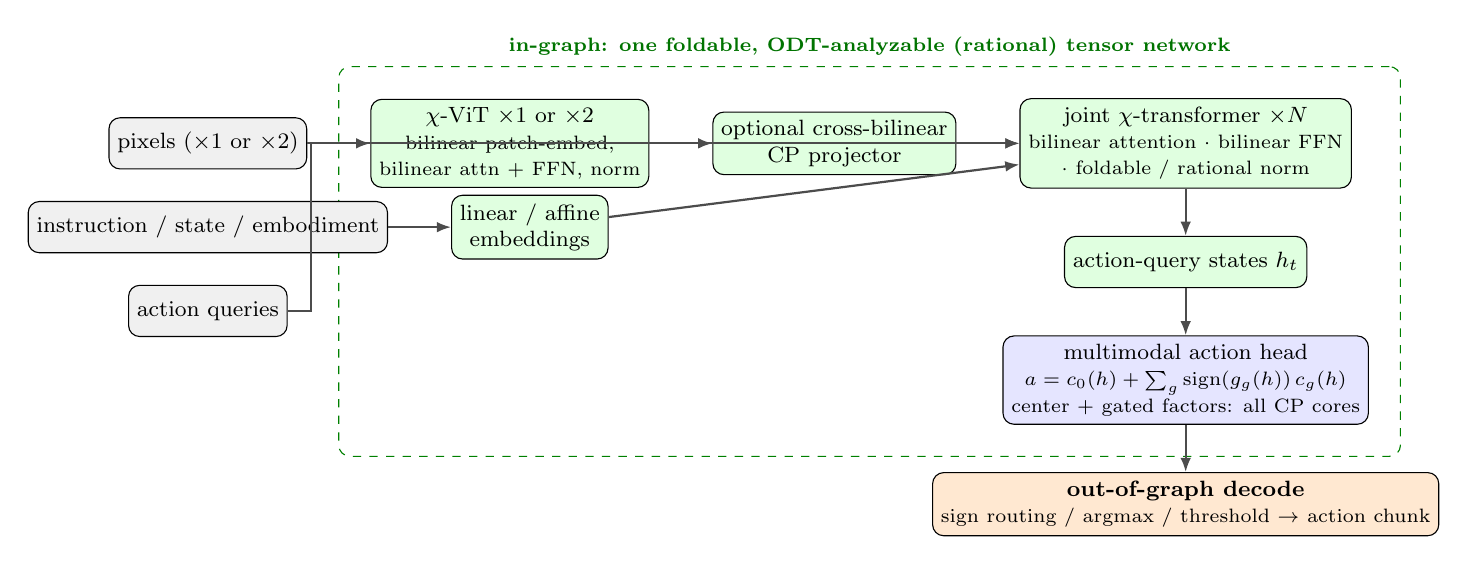
\begin{tikzpicture}[
  font=\footnotesize,
  box/.style={draw, rounded corners, align=center, minimum height=6.5mm, inner sep=3pt},
  inp/.style={box, fill=gray!12},
  prim/.style={box, fill=green!12},
  head/.style={box, fill=blue!10},
  dec/.style={box, fill=orange!18},
  arr/.style={-{Latex[length=1.8mm]}, thick, gray!60!black},
  node distance=4mm and 8mm,
]
% inputs (left)
\node[inp] (img) {pixels ($\times 1$ or $\times 2$)};
\node[inp, below=of img] (lang) {instruction / state / embodiment};
\node[inp, below=of lang] (aq) {action queries};
% encoders
\node[prim, right=of img] (vit) {$\chi$-ViT $\times 1$ or $\times 2$\\{\scriptsize bilinear patch-embed,}\\{\scriptsize bilinear attn + FFN, norm}};
\node[prim, right=of vit] (proj) {optional cross-bilinear\\CP projector};
\node[prim, right=of lang] (emb) {linear / affine\\embeddings};
% backbone (spanning)
\node[prim, right=8mm of proj, minimum width=34mm] (bb) {joint $\chi$-transformer $\times N$\\{\scriptsize bilinear attention $\cdot$ bilinear FFN}\\{\scriptsize $\cdot$ foldable / rational norm}};
% action-query states
\node[box, fill=green!12, below=6mm of bb] (h) {action-query states $h_t$};
% multimodal head
\node[head, below=6mm of h] (mh) {multimodal action head\\{\scriptsize $a=c_0(h)+\sum_g \mathrm{sign}(g_g(h))\,c_g(h)$}\\{\scriptsize center + gated factors: all CP cores}};
% decode (outside)
\node[dec, below=6mm of mh] (dec) {\textbf{out-of-graph decode}\\{\scriptsize sign routing / argmax / threshold $\to$ action chunk}};
% arrows
\draw[arr] (img) -- (vit); \draw[arr] (vit) -- (proj); \draw[arr] (proj) -- (bb);
\draw[arr] (lang) -- (emb); \draw[arr] (emb) -- (bb);
\draw[arr] (aq.east) -- ++(3mm,0) |- (bb.west);
\draw[arr] (bb) -- (h); \draw[arr] (h) -- (mh); \draw[arr] (mh) -- (dec);
% in-graph shaded boundary around everything except the decode
\begin{scope}[on background layer]
\node[draw=green!50!black, dashed, rounded corners, fit=(vit)(proj)(emb)(bb)(h)(mh),
      inner sep=4mm, label={[green!45!black,font=\scriptsize\bfseries]above:in-graph: one foldable, ODT-analyzable (rational) tensor network}] {};
\end{scope}
\end{tikzpicture}
}
\caption{\textbf{$\chi$-VLA internal dataflow and the tensor-network boundary.} In the
general two-view configuration, every learned block, both vision $\chi$-ViTs, the
cross-bilinear CP fusion projector, the
linear/affine embeddings, the joint $\chi$-transformer (bilinear attention $+$ bilinear FFN
$+$ foldable-scalar or exact rational per-instance normalization), and the multimodal action
head (a mixture of CP cores), is a polynomial or rational tensor primitive, so the whole
map folds into a single ODT-analyzable tensor network (dashed box). Only the final
\emph{decode} (sign routing for the mode, or an argmax/threshold) is a non-polynomial
controller op, applied \emph{outside} the network, the same status OpenVLA gives its
argmax. The learned action \emph{distribution} stays in-graph. Only the selection leaves it.
The $94.2\%$ checkpoint uses the simpler single-view path, no fusion projector, and a linear
action head, detailed in Table~\ref{tab:closedloop-config}.}
\label{fig:arch-detail}
\end{figure}

\paragraph{Foldability is achievable but requires care (details in
Appendix~\ref{app:stability}).} Making the scalar (foldable) normalization stable inside a
deep degree-two stack requires keeping residual branches near the identity (small learned
gains, initialized at $0.01$) and distilling from a stable per-token teacher. The resulting
student matches its teacher and folds to a normalization-free graph to $10^{-6}$ (fp32) /
$10^{-12}$ (fp64). Per-instance normalization need not even be approximated by a frozen
scalar: carried in projective (numerator, denominator) coordinates it folds \emph{exactly}
as a rational tensor network $P(x)/Q(x)$ (both $P,Q$ polynomial/CP), verified to $10^{-14}$
(\S\ref{sec:discussion}), so the substrate spans the rational, not merely polynomial,
tensor-network class. This is an engineering prerequisite, orthogonal to the interpretability
findings that follow.

% ============================================================================
\section{Recovering capability inside the tensor network}
\label{sec:capability}
% ============================================================================

Two operations a capable policy needs are inherently nonlinear, and a naive bilinear
replacement either collapses (the action head) or only approximates (normalization). This
section gives the constructions that recover both while keeping the learned map a single
tensor network, with the mathematics of how each works. The organizing principle is a
boundary. The learned \emph{distribution} stays in-graph and polynomial or rational, and only
the final \emph{decode} (a selection) is a controller operation outside the network, exactly
the status OpenVLA gives its argmax.

\subsection{Why a linear action head collapses}
The default head is a linear map $\hat a = W_a h + b_a$ of the post-attention action-query
state $h$, trained by mean-squared error. For a fixed observation the minimizer of
$\mathbb{E}\,\|a-\hat a\|^2$ is the conditional mean $\mathbb{E}[a\mid h]$. When the
demonstrations are multimodal, meaning the same $h$ admits several valid actions, that mean is
an average of valid behaviours and is usually itself invalid. The gripper command
$\in\{-1,+1\}$ averages to $\approx 0$ (it never commits to a grasp), and two arm approaches
average to a path between them. On LIBERO-Object about $40\%$ of near-identical-observation
neighbourhoods are genuinely bimodal (Section~\ref{sec:discussion}), so this is the common
case, not a corner case.

\subsection{The product-routing multimodal head}
Read the pooled action-query state $h\in\mathbb{R}^{d}$. Define one \emph{center} core, $G$
\emph{factor} cores, and $G$ scalar \emph{gate} cores, each the bilinear (CP) primitive
$\mathrm{BFFN}(x)=D[(L\bar x)\otimes(R\bar x)]$ of $h$:
\begin{equation}
c_0(h)\in\mathbb{R}^{m}, \qquad c_g(h)\in\mathbb{R}^{m}, \qquad g_g(h)\in\mathbb{R},
\qquad g=1,\dots,G,
\end{equation}
where $m=H\,d_a$ is the flattened action chunk ($H$ steps of dimension $d_a$). A binary code
$b\in\{0,1\}^{G}$ selects an action
\begin{equation}
a(h,b) = c_0(h) + \sum_{g=1}^{G}(2b_g-1)\,c_g(h).
\label{eq:zonotope}
\end{equation}
As $b$ ranges over $\{0,1\}^{G}$, Eq.~\eqref{eq:zonotope} traces the $2^{G}$ vertices of a
$G$-dimensional zonotope centered at $c_0(h)$ with edge vectors $\pm c_g(h)$. It is a mixture
of $2^{G}$ modes built from only $2G+1$ CP cores, so the number of representable modes is
exponential in the core count. Because every core is a $\mathrm{BFFN}$, the map
$h\mapsto\{c_0,c_g,g_g\}$ folds into the tensor network exactly, with fold error
$\sim 4\times 10^{-16}$.

\paragraph{Decode (out-of-graph).} At inference the mode is chosen by the sign of each gate,
\begin{equation}
\hat b_g = \mathbf{1}[\,g_g(h)>0\,], \qquad \hat a = a(h,\hat b),
\end{equation}
a winner-take-all controller operation outside the network. A soft average
$\sum_b \pi_b(h)\,a(h,b)$ would re-collapse to the conditional mean, the very failure being
escaped, so the decode commits to one mode. This is the same category of external operation as
OpenVLA's token argmax and our gripper threshold.

\subsection{Training the head without losing precision}
Assigning each demonstration only to its best mode is high-variance and, on the majority of
states that are effectively unimodal, less precise than a plain mean regressor. We keep
precision with two loss-only additions. For a demonstration $a^{*}$ the best code is
\begin{equation}
b^{*} = \arg\min_{b\in\{0,1\}^{G}} \|a(h,b)-a^{*}\|^2,
\end{equation}
found by enumeration for small $G$. The loss combines a temperature-annealed soft assignment,
a gate cross-entropy, and a distillation anchor to an auxiliary linear teacher $\mu_T(h)$:
\begin{equation}
\mathcal{L} = \sum_{b} w_b(\tau)\,\|a(h,b)-a^{*}\|^2
\;+\; \lambda_{\mathrm{gate}}\,\mathrm{BCE}\!\big(g(h),\,b^{*}\big)
\;+\; \lambda_{\mathrm{distill}}\,\|c_0(h)-\mu_T(h)\|^2 ,
\label{eq:headloss}
\end{equation}
with $w_b(\tau)=\mathrm{softmax}\big(-\|a(h,b)-a^{*}\|^2/\tau\big)$ and the temperature $\tau$
annealed from soft (a re-averaging regime that fits the mean precisely, like the linear head)
to hard (full commitment). The distillation term pulls the mixture center onto the precise
conditional mean on unimodal states, so the head degrades gracefully to the linear head where
there is no multimodality and branches only where there is. Every non-polynomial operation
(the $\arg\min$, the softmax weights, the sign decode) is confined to the loss or the decode.
The deployed forward map is a polynomial tensor network.

\begin{figure}[t]
\centering
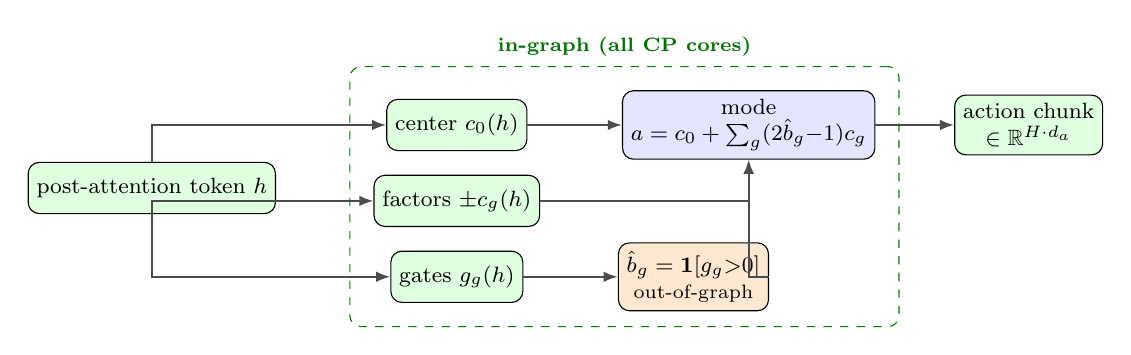
\begin{tikzpicture}[
  font=\footnotesize,
  box/.style={draw, rounded corners, align=center, minimum height=6.5mm, inner sep=3pt},
  prim/.style={box, fill=green!12},
  dec/.style={box, fill=orange!18},
  sel/.style={box, fill=blue!10},
  arr/.style={-{Latex[length=1.8mm]}, thick, gray!60!black},
]
\node[box, fill=green!12] (h) {post-attention token $h$};
\node[prim, right=14mm of h, yshift=8mm] (c0) {center $c_0(h)$};
\node[prim, below=3mm of c0] (cg) {factors $\pm c_g(h)$};
\node[prim, below=3mm of cg] (gg) {gates $g_g(h)$};
\node[dec, right=12mm of gg] (sign) {$\hat b_g=\mathbf{1}[g_g{>}0]$\\{\scriptsize out-of-graph}};
\node[sel, right=12mm of c0] (mode) {mode\\$a=c_0+\sum_g(2\hat b_g{-}1)c_g$};
\node[box, fill=green!12, right=10mm of mode] (out) {action chunk\\$\in\mathbb{R}^{H\cdot d_a}$};
\draw[arr] (h) |- (c0); \draw[arr] (h) |- (cg); \draw[arr] (h) |- (gg);
\draw[arr] (gg) -- (sign);
\draw[arr] (c0) -- (mode); \draw[arr] (cg) -| (mode);
\draw[arr] (sign) -| (mode);
\draw[arr] (mode) -- (out);
\begin{scope}[on background layer]
\node[draw=green!50!black, dashed, rounded corners, fit=(c0)(cg)(gg)(mode),
      inner sep=3mm, label={[green!45!black,font=\scriptsize\bfseries]above:in-graph (all CP cores)}] {};
\end{scope}
\end{tikzpicture}
\caption{\textbf{The product-routing multimodal action head.} From the post-attention token
$h$, a center core, $G$ factor cores, and $G$ scalar gate cores (all bilinear CP maps) define a
mixture over $2^{G}$ zonotope-vertex modes (Eq.~\ref{eq:zonotope}). Everything inside the
dashed box is polynomial and folds exactly. Only the gate \emph{sign} that picks the mode is a
non-polynomial controller operation, applied outside the network.}
\label{fig:head}
\end{figure}

With this head the policy commits to a mode instead of averaging. In the earlier
short-training protocol the curriculum and distillation variant reached
$44\%\pm30\%$ over five seeds, with individual seeds from $0\%$ to $82.5\%$, while the
linear-mean head reached about $19\%\pm15\%$ over three seeds. The ranges overlap, so these
results establish non-trivial closed-loop control but not a reliable advantage over the
linear head.

\subsection{Exact per-instance normalization as a rational tensor network}
\label{subsec:rationalnorm}
The remaining inherently nonlinear component is per-instance normalization. RMS normalization
$n(x)=x/\sqrt{\mathbb{E}[x^2]+\epsilon}$ divides by a statistic of its own input, which the
strict polynomial scheme approximates by a frozen scalar (Appendix~\ref{app:stability}). The
approximation is avoidable. Carry each activation in projective coordinates $(N,D)$ standing
for the value $N/D$. A linear map acts as $(N,D)\mapsto(WN,D)$ and a bilinear core as
$(N,D)\mapsto\big((LN)\otimes(RN),\,D^{2}\big)$, so a per-instance normalization whose divisor
is a \emph{polynomial} of the activation (for example the mean square $\mathbb{E}[x^2]+\epsilon$,
which has no square root) never requires a mid-network division. The whole network becomes a
ratio $P(x)/Q(x)$ of two polynomial (CP) tensor networks. Both fold and are ODT-analyzable,
with $Q$ the activation-energy form. A bilinear stack with per-instance mean-square
normalization reproduces its projective fold to $10^{-14}$. This exact result applies to
division by mean square, not to true RMS normalization. The square root in RMS is algebraic
rather than rational. We therefore implement either the exact mean-square variant or a fixed
rational approximation of $1/\sqrt{\cdot}$. The latter is an approximation to RMSNorm, while
its deployed map is exactly a rational function and can be represented by a rational tensor
network. In operator tests it differs from per-token RMSNorm by less than $1\%$ over the
measured activation range. Retraining the complete policy with this rational operator at every
block and attention QK normalization site reaches $94.5\%$ ($189/200$) over all ten
LIBERO-Object tasks in one seed (\S\ref{sec:substrate}).

\subsection{Verifying decomposability on the trained policy, not just architecturally}
\label{subsec:decompaudit}

Everything above is an architectural argument, every primitive we assemble is individually
polynomial or rational. Whether the \emph{actual trained} $189/200$ checkpoint is decomposable
is a separate, empirical question, and we check it directly, on the real weights and real
held-out LIBERO-Object frames (no synthetic data, no toy network).

\paragraph{(i) A mechanical purity audit.} We walk every module instance the trained policy
actually invokes on a forward pass and check membership in the allowed set
$\{\text{Linear}, \text{Embedding}, \text{Conv2d(patch-embed)}, \mathrm{BFFN}, \text{bilinear
attention}, \text{RationalNorm}\}$, and separately assert the absence of any frozen-scalar,
per-token, or homotopy normalization instance and of any softmax/GELU/ReLU/LayerNorm module.
The audit finds $112$ \texttt{Linear}, $74$ \texttt{RationalNorm}, $2$ \texttt{Embedding}, and
$1$ \texttt{Conv2d} (the fixed-stride patch embed) leaf modules, and zero forbidden types: a
certificate, not an architectural claim.

\paragraph{(ii) Exact projective fold-and-verify on real weights.} We take one backbone block's
$\mathrm{RationalNorm}\!\to\!\mathrm{BFFN}$ branch from the trained checkpoint and reconstruct
it as a literal ratio of two polynomial tensor networks on $54{,}784$ real activation rows
(held-out frames, propagated through the real trained attention sub-layer to reach this branch's
actual input distribution). $\mathrm{BFFN}$'s exact cubic core $T$ (\S\ref{sec:capability}) gives
the numerator network directly; the $\mathrm{RationalNorm}$ forward pass is algebraically
rearranged into projective (numerator, denominator) form (\S\ref{subsec:rationalnorm}) using its
own trained coefficients. The reconstruction is computed in native double precision throughout.
Compared against the real deployed \texttt{forward()} (which internally computes its per-instance
statistic in float32 by design, independent of caller precision), the median relative
discrepancy is $1.4\times10^{-7}$, at the float32 precision floor, not evidence of any
approximation in the rational algebra itself. (iii) \textbf{Whole-model fp64/fp32 determinism.}
Running the full trained policy at double versus single precision on the same real inputs gives
a maximum output discrepancy of $2.2\times10^{-3}$ on an action scale of $\sim$$0.74$
($\sim$$0.3\%$ relative), consistent with ordinary floating-point rounding compounding over eight
layers, not any hidden non-algebraic behaviour (a branch, a lookup, a numerical solver).

\paragraph{Honest scope.} This verifies decomposability \emph{mechanically and representatively}
on the trained model, not \emph{exhaustively}: explicitly materializing one global polynomial for
the entire attention-crossing network remains combinatorially infeasible, exactly as
\S\ref{subsec:attndepth} already explains, and is not what is newly shown here. What is new is
that every operation actually used by the trained $189/200$ policy is confirmed, by a mechanical
walk of the real module graph plus an exact reconstruction on real trained weights, to belong to
the polynomial/rational class, closing the paper's earlier open item that a materialized
rational export on the real policy remained unverified.

% ============================================================================
\section{Exact global decomposition (ODT), in depth}
\label{sec:odt}
% ============================================================================

This section is the payoff of the whole design and we treat it carefully. An
ordinary softmax-and-normalization policy cannot be turned into a single algebraic
object, so it cannot be globally diagonalized. A tensor network can.

\subsection{What ODT is, and why it needs a tensor network}

Suppose we want to compress a network by discarding directions in one of its
hidden spaces, keeping only the ones that matter for the output. Call the hidden
space we are analyzing a ``bond''. The naive approach is a local one: take the
weight matrix that reads from that bond, run a singular value decomposition (SVD),
and keep its top directions. This is greedy and per-layer. It only sees the one
adjacent weight matrix, not what the rest of the network does with those
directions downstream.

Orthogonalize-Diagonalize-Truncate (ODT), introduced for tree-shaped bilinear
networks by Dooms et al. \cite{chinets}, instead ranks bond directions by their
\emph{global} importance, accounting for the entire rest of the network, which we
call the ``environment'' of the bond. This is only possible if the whole model is
one multilinear object, because only then can the environment be contracted into a
single operator whose singular directions are the true global importances. The
three steps are:

\begin{enumerate}
  \item \textbf{Orthogonalize.} Sweep through the network and replace each weight
  core by an isometry (an orthonormal map) times a small triangular remainder,
  using a reduced RQ decomposition of the matricized core, pushing the remainder
  toward the output. After this sweep each bond has an orthonormal basis, so
  importance can be read off directly as singular values rather than being tangled
  up with the basis.
  \item \textbf{Diagonalize.} At a bond, form the Gram matrix of the environment,
  $G = Q^{*}Q$, where $Q$ is the downstream map from the bond to the output. Its
  eigenvalues are the squared global importances of the bond directions and its
  eigenvectors are those directions.
  \item \textbf{Truncate.} Keep the top $k$ eigenvectors, insert the projector
  $P_k = V_kV_k^{\top}$ at the bond, and absorb it into the adjacent cores. The
  output error is bounded by the square root of the sum of the discarded
  eigenvalues, so the spectrum tells you in advance how much you can remove.
\end{enumerate}

\subsection{How we compute it for a bilinear chain}

Our exact-decomposition model is a feed-forward bilinear network we call a
$\chi$-MLP, chosen because a chain with no attention and no residual connection is
a clean tree, exactly the setting ODT was designed for. After folding, it is
\begin{equation}
z_0 = [1;\,Ex], \qquad a_i = C_i(z_{i-1},z_{i-1}), \qquad z_i = [1;\,a_i],
\qquad \text{logits} = W_{\text{head}}\,a_L + b,
\end{equation}
where $E$ is a linear input embedding, each $C_i\in\mathbb{R}^{d\times(d+1)\times(d+1)}$
is a symmetric bilinear core recovered from the folded layer, and $C_i(z,z)$ means
contracting the core twice with the homogeneous activation $z$.

To rank the directions of a bond $a_i$ by global importance we build the exact
downstream map from $a_i$ to the output and contract it against itself over the
output index and over every environment leg, leaving the bond leg open on both
sides. For the deepest bond (the output of the first layer, whose downstream is two
more bilinear layers) the downstream is a degree-four form in $z_i$. We construct
it explicitly by composing the cores,
\begin{equation}
D[c,i,j,k,l] = \sum_{p,q} C^{\text{head}}_L[c,p,q]\; Z_2[p,i,j]\; Z_2[q,k,l],
\qquad
G[i,i'] = \sum_{c,j,k,l} D[c,i,j,k,l]\,D[c,i',j,k,l],
\end{equation}
where $Z_2$ expresses the second-layer homogeneous activation as a quadratic form
in $z_i$ and $C^{\text{head}}_L$ folds the linear head into the last core. The
$d\times d$ block of $G$ over the non-constant coordinates gives the global
importances. The local baseline uses only the adjacent core (the layer that
directly reads the bond), ignoring everything downstream. Truncation projects the
activation onto the top $k$ eigenvectors and we measure the resulting accuracy.

\subsection{Results on the $\chi$-MLP}

We train a three-layer $\chi$-MLP (bond width $32$) on the SVHN digit dataset to
$0.81$ accuracy and run the exact procedure.

\begin{itemize}
  \item \textbf{Exact reconstruction.} The unrolled tensor network reproduces the
  trained module to $5\times10^{-12}$ in double precision, confirming that the
  exported cores are the model, not an approximation of it.
  \item \textbf{Global low-rank structure.} Ranking the deepest bond by the global
  Gram, $20$ of its $32$ hidden dimensions ($62\%$) can be removed with at most a
  $1\%$ accuracy drop. Dooms et al. report about $70\%$ on their own SVHN network. We report our measured figure rather than assuming their number transfers.
  \item \textbf{Global beats local.} At a matched number of kept directions, the
  global ranking preserves accuracy better than the local per-layer SVD, most
  clearly at the compression elbow.
\end{itemize}

\begin{center}\small
\begin{tabular}{@{}lcccccc@{}}
\toprule
retained directions $k$ & 4 & 6 & 8 & 12 & 16 \\ \midrule
global ODT  & 0.571 & \textbf{0.777} & 0.797 & 0.809 & 0.811 \\
local SVD   & 0.523 & 0.686 & 0.798 & 0.807 & 0.811 \\
\bottomrule
\end{tabular}\quad (full width $32$ gives $0.808$. Deepest bond)
\end{center}

The reason global wins is exactly the reason it needs a tensor network: at $k=6$
the global ranking already knows which directions the two downstream layers will
actually use, while the local ranking only sees the immediately following layer
and keeps directions that later turn out not to matter.

\subsection{From compression to interpretation: are the ranked modes real?}

Removable-dimension counts show that low-rank structure \emph{exists}. They do not
show that the surviving directions are human-interpretable, nor that the ranking is
\emph{causal} rather than merely a good compressor. D\'eh\'erand \cite{deherand}
takes the complementary step, extending the $\chi$-net idea to convolutional
networks and reading each class output as a quadratic form whose eigenvectors,
projected to pixels, are spatially coherent digit strokes. Two things are left
open there: the interpretation is run only on a shallow single-bilinear layer, and
visual coherence is never tied to an intervention. We close both on our own models.

\paragraph{Output-conditioned atoms.} For a classifier with one bilinear layer, each
class logit is \emph{exactly} a quadratic form in the homogeneous embedded input,
$\ell_c(x)=z^\top Q_c\,z+b_c$ with $z=[1;Ex]$ and $Q_c=\sum_o W^{\text{head}}_{c,o}C_o$
the head folded into the core (reconstruction against the trained module is
$2.6\times10^{-13}$ on SVHN, $0.80$ accuracy). Eigendecomposing $Q_c=\sum_i\lambda_i
v_iv_i^\top$ writes the logit as $\sum_i\lambda_i(v_i\!\cdot\! z)^2+b_c$: signed
``atoms'' where $\lambda_i>0$ supports class $c$ and $\lambda_i<0$ suppresses it,
each projected to a pixel sensitivity map through $E$.

\begin{figure}[t]
\centering
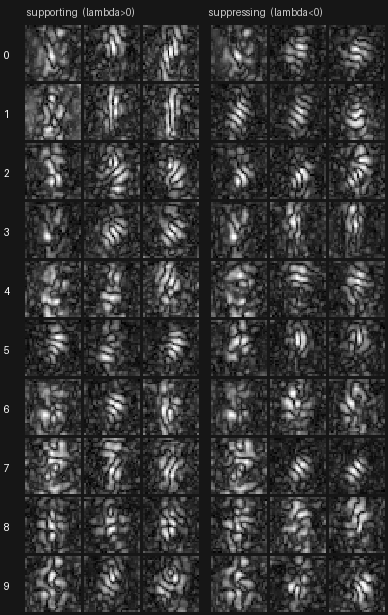
\includegraphics[width=0.62\textwidth]{odt_atoms_shallow.png}\\[4pt]
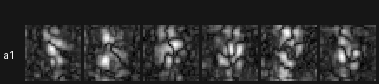
\includegraphics[width=0.82\textwidth]{odt_atoms_deep.png}
\caption{Extracted ODT eigen-atoms projected to pixels (brighter = higher
sensitivity). \textbf{Top:} the single-bilinear $\chi$-classifier, one row per SVHN
class. The three left atoms of each row \emph{support} the class ($\lambda>0$), the
three right \emph{suppress} it ($\lambda<0$). \textbf{Bottom:} the six top global
directions of the deep three-layer $\chi$-MLP. The atoms are causal and
class-relevant. How \emph{localized} they are depends on architecture topology, which
we quantify across dense/convolutional/locally-connected models in
Section~\ref{sec:findings}.}
\label{fig:atoms}
\end{figure}

These atoms (Figure~\ref{fig:atoms}) are the object analyzed in
Section~\ref{sec:findings}, where we ask the three questions this section motivates:
is the ranking \emph{causal} (deletion/insertion faithfulness against integrated
gradients and PCA), are the atoms \emph{coherent} (a function of topology, not
convertibility), and, for a policy, at which \emph{bond} is the mechanism
readable and controllable. We turn to those results next.

\subsection{Does this survive attention and residual connections?}
\label{subsec:attndepth}

The $\chi$-MLP is feed-forward. A transformer adds attention (which mixes
information across token positions) and residual connections. Extending exact,
weight-only global ODT to a general attention network is an open problem, because
the attention pattern is itself a learned degree-four function of the inputs, so
the environment is no longer a fixed operator. We give the first empirical
evidence that the structure is nonetheless there.

We train a strict, foldable transformer language model (using the
teacher-then-distill recipe so it is stable) and analyze the bond at the block
input, whose downstream \emph{crosses} the attention layer (each token feeds the
queries, keys, and values of every position), then the residual path, the
feed-forward layer, and the head. Because the attention pattern is data-dependent
here, we rank directions by a data-driven version of the global Gram, the average
outer product of the output gradient at the bond, which measures how much each
direction of the bond actually affects the loss through the full downstream
including attention. The local baseline is the SVD of the adjacent input
projections (the query, key, value, and feed-forward input weights).

\begin{center}\small
\begin{tabular}{@{}lccc@{}}
\toprule
 & retained $k$ & global (output-aware) & local (weight SVD) \\ \midrule
\textbf{1 attention layer} (full-rank loss $5.23$) & 32 & \textbf{6.11} & 7.88 \\
                                                    & 64 & \textbf{5.47} & 6.27 \\
                                                    & 96 & \textbf{5.27} & 5.55 \\
\midrule
\textbf{2 attention layers} (full-rank loss $5.98$) & 32 & \textbf{6.18} & 7.78 \\
                                                    & 64 & \textbf{6.02} & 6.52 \\
                                                    & 96 & \textbf{5.99} & 6.18 \\
\bottomrule
\end{tabular}
\end{center}

The global ranking beats the local one at every retained width for both models,
and the attention model still folds to an exact tensor network (double-precision
fold error at machine precision). Notably the two-layer model is \emph{more}
compressible ($64$ of $128$ directions, $50\%$, removable at under $0.05$ nats)
than the one-layer model ($25\%$), which suggests deeper attention stacks have
more, not less, global low-rank structure. Two honest caveats. First, this uses
the data-driven global Gram. The fully weight-based, data-free contraction across
an attention-crossing bond, and the transfer of the tree error bound, remain open.
For bonds whose downstream is feed-forward (for example, the bond after the
attention sub-layer), the exact weight-based procedure of the previous subsection
applies directly. Second, the strict scalar-normalization model needs the
distillation recipe to train stably beyond one layer.

\subsection{Cost and limits}

For the tree network the procedure costs about $O(Lh^4)$ time with $O(h^3)$ memory
in the bond width $h$, which is why our exact-decomposition models use a small
width. Unrolling a full attention transformer into one tensor over all token
positions grows combinatorially, so exact whole-model contraction is only feasible
at small scale. The practical path is to decompose one analysis bond at a time, as
above.

\section{What decomposability buys: causality, topology, and bonds}
\label{sec:findings}

The previous section established that the exported bilinear network can be exactly
decomposed and that a global ODT ranking is meaningful. Here we ask the sharper question:
\emph{how much of ``interpretability'' does that decomposability actually buy?} It buys a
causal, rankable basis, but coherence and nameability are bought separately, by topology
and by bond placement.

\subsection{Causality is competitive with standard attribution, and (at feed-forward bonds) free}

We compare the ODT direction ranking against real baselines, unsupervised PCA of
activations, integrated gradients \cite{ig}, and random, using deletion/insertion
faithfulness AUC (project the input/bond onto, or out of, the top-$k$ directions and measure
accuracy). On the softmax-free \chivit\ (patch bond, downstream crossing all attention
layers) and on an exact feed-forward classifier:

\begin{center}\small
\begin{tabular}{@{}llcc@{}}
\toprule
substrate & ranking & deletion AUC $\downarrow$ & insertion AUC $\uparrow$ \\ \midrule
\chivit\ (attn) & ODT (ours) & 0.150 & 0.792 \\
                & PCA        & 0.151 & 0.788 \\
                & random     & 0.498 & 0.491 \\ \midrule
classifier      & ODT (\textbf{data-free}) & 0.222 & 0.786 \\
                & integrated gradients     & 0.191 & 0.784 \\
                & PCA                      & 0.204 & 0.800 \\
                & random                   & 0.548 & 0.530 \\
\bottomrule
\end{tabular}\quad(3 / 2 seeds. Std $\le 0.03$)
\end{center}

The ODT ranking is strongly faithful, it crushes random, and is \emph{competitive
with}, not superior to, PCA and integrated gradients. Its distinctive properties are that it
is \emph{weight-derived} (at feed-forward bonds it needs no data at all, unlike PCA and
integrated gradients) and \emph{globally rankable} (integrated gradients is per-sample).
Through attention we fall back to a data-driven output-sensitivity Gram, so the ``for free''
claim is honest only at feed-forward bonds. The causal structure nonetheless survives
attention (the \chivit\ bond above crosses four attention layers) and, in our small
models, appears to grow \emph{more} compressible with depth
(Section~\ref{subsec:attndepth}). Reassuringly, the two bases largely agree where both are
computable: on the feed-forward classifier the exact weight-only basis and the data-driven
Gram basis have top-$64$ subspace overlap $0.53$ (rising to $0.65$ at $256$) versus a random
baseline of $0.02$--$0.08$, so the data-driven Gram used through attention is a faithful
proxy for the weight-only method, not a different object.

\subsection{Coherence is bought by topology, at no capability cost}
\label{subsec:topology}

Whether the causal directions are \emph{human-coherent} (localized, nameable) is not a
property of convertibility, it is set by architecture topology. On single-bilinear
classifiers whose class logit is exactly a quadratic form, we measure eigen-atom spatial
locality (energy in the top $10\%$ of pixels, relative to random directions), across three
seeds and two datasets:

\begin{center}\small
\begin{tabular}{@{}lcccc@{}}
\toprule
 & \multicolumn{2}{c}{SVHN} & \multicolumn{2}{c}{CIFAR-10} \\
architecture & acc & locality ($\times$rand) & acc & locality ($\times$rand) \\ \midrule
dense                 & $0.747$ & $2.29$ & $0.354$ & $1.47$ \\
conv (spatial readout)& $\mathbf{0.814}$ & $\mathbf{3.45}$ & $\mathbf{0.630}$ & $3.42$ \\
locally-connected     & $0.800$ & $3.48$ & $0.584$ & $\mathbf{3.44}$ \\
\bottomrule
\end{tabular}\quad(mean over 3 seeds, std $\le 0.05$)
\end{center}

Spatial-locality-preserving topology reaches $\sim$$3.5\times$ random-baseline locality on
both datasets, versus $2.29$ (SVHN) / $1.47$ (CIFAR) for dense, i.e.\ $\sim$$1.5$--$2.3\times$
more localized than dense, and the gap is \emph{larger} on the harder dataset. The effect is
not a capacity confound. A width sweep ($8\!\to\!128$) shows dense locality is
\emph{capacity-independent}: growing the dense model raises accuracy ($0.70\!\to\!0.75$) but
its atom locality stays flat at $\sim$$2.2$, never approaching the $\sim$$3.5$ of the
structured topologies at any width, so coherence is set by topology, not parameters or
accuracy (and the most coherent model is also the most accurate and parameter-efficient). A
deep-network replication (data-driven input-space ranking, depth 1 vs 3) shows the gap
survives depth and \emph{strengthens} with it (conv locality $2.05\!\to\!2.52$ on CIFAR while
dense stays $\sim$$1.4$). It also holds \emph{beyond} $32\times32$: on STL-10 at $64\times64$,
conv atoms remain more localized than dense ($1.88$ vs $1.41$) and conv is more accurate ($0.45$
vs $0.32$), with the same causal global$\gg$random ranking. One honest subtlety: plain
convolution with \emph{global} pooling
underperforms, global pooling imposes translation-invariance that both starves capacity
and delocalizes modes. The spatial readout recovers both.

\subsection{For a policy, mechanisms live behind the attention}

On \chivla\ (the synthetic reach task), the action-relevant quantity is which object the
instruction names and where it is. This must be \emph{constructed} by attention (bind the
named identity to a location), and indeed it is not linearly present at the network input but
is at the post-attention action-query bond:

\begin{center}\small
\begin{tabular}{@{}lcc@{}}
\toprule
quantity (linear decodability) & input bond & post-attention bond \\ \midrule
target position $x$/$y$ ($R^2$, 3 seeds) & $0.20{\scriptstyle\pm.01}$ & $\mathbf{0.92{\scriptstyle\pm.03}}$ \\
gripper position (in the state token) & $0.99$ & $0.97$ \\
named colour / shape (in the instruction) & $1.00$ & $0.94$ \\
\bottomrule
\end{tabular}
\end{center}

Only the \emph{bound} quantity (target position) jumps across the attention. The raw
ingredients are linear at both bonds. We then verify the mechanism is \emph{causal} with an
intervention: rewriting the instruction to name a different present object (image and state
fixed) makes the predicted action follow the new target, with $R^2 = 0.956\pm0.016$ and a
$97.1\%$ switch-rate (3 seeds). Notably a purely \emph{correlational} handle fails, patching
the linear target-position \emph{decode} direction does not steer the action (transfer $0.002$
vs $0.012$ for random), an instance of the decode-is-not-control gap \cite{amnesic} that
motivates causal over correlational interpretation.

\subsection{Interpretability on the real, closed-loop-competitive policy}
\label{subsec:realpolicyodt}

The results above are on components (a classifier, a ViT, a synthetic reach policy). We close
the loop on the actual object: the trained, rational-by-construction, closed-loop
LIBERO-Object policy
(rational per-instance norm throughout, \S\ref{subsec:rationalnorm}; capability numbers in
\S\ref{sec:substrate}). We build a data-driven output-sensitivity Gram at the
\emph{visual-patch} bond (downstream of the bond: the entire causal bilinear-attention backbone
plus the linear action head) for each action group -- end-effector translation, rotation,
gripper -- from $\sim$$2000$ held-out frames (no training, no simulation), then truncate the
bond onto its top-$k$ \emph{global} eigendirections versus a random $k$-subspace and measure the
offline action reconstruction error:

\begin{center}\small
\begin{tabular}{@{}lccc@{}}
\toprule
group ($k{=}64$ of $384$, $\sim$$17\%$) & global MSE & random MSE & ratio \\ \midrule
end-effector translation & $0.058$ & $0.276$ & $4.8\times$ \\
rotation & $0.121$ & $0.561$ & $4.6\times$ \\
gripper & $0.007$ & $0.280$ & $\mathbf{42\times}$ \\
\bottomrule
\end{tabular}
\end{center}

The action-relevant computation is globally low-rank and causally rankable on the real,
deployed policy, not just on a classifier or a synthetic task -- extending the
convertibility-buys-causality claim to the artifact that actually matters. (Honest nuance: at
very small $k$ ($4$--$8$) global and random are comparable or global is slightly worse for the
translation/rotation groups, plausibly because the top eigendirections of a Gram aggregated
over heterogeneous multi-task demonstrations mix across tasks; the causal ranking becomes
decisive from $k{\approx}32$ upward, which is also the regime where the $4$--$42\times$ headline
holds.) We separately measure \emph{coherence}: for each group's top causal direction, the
fraction of energy concentrated in the most-activated $10\%$ of the $8{\times}8$ patch grid,
against $30$ random directions. The result is modest, not dramatic ($1.08$--$1.41\times$
random), consistent with the topology finding above (\S\ref{subsec:topology}): a
\emph{dense}, from-scratch patch embedding gives causal-but-diffuse mechanisms, and spatial
coherence would need a locality-preserving (e.g.\ convolutional) vision encoder -- a prediction
for future work, not yet tested on this real policy.

\subsection{A real causal intervention in the live simulator: an honest negative}
\label{subsec:realintervention}

The results above are correlational sensitivity measures (truncate a bond, watch the offline
error). The stronger causal test, in the spirit of the synthetic-task intervention
(\S\ref{sec:findings}, $R^2=0.956$, switch-rate $97.1\%$), is a real behavioural manipulation:
does changing what the instruction \emph{names} change what the policy \emph{does}? Every
LIBERO-Object scene contains several co-present distractor grocery items alongside the true
target (confirmed directly from the simulator state), so we can hold the image and robot state
fixed and only swap the instruction to name a distractor already in the scene, then compare the
policy's predicted first-step reach direction against the true 3D direction (known exactly from
simulator state) to the original target and to the newly-named object, over $32$ (task,
distractor) trials across eight tasks.

The result is an honest negative. Under the true instruction the predicted direction correlates
with the true target reasonably well (mean cosine similarity $0.474$). Under the swapped
instruction it correlates only weakly with the newly-named object ($0.313$) and, tellingly,
\emph{still more} with the original target ($0.395$): the switch rate (direction becomes
better-aligned with whichever object is named) is only $15.6\%$, far short of the synthetic
task's $97.1\%$. We do not read this as evidence against the causal, low-rank structure measured
above, offline truncation faithfulness and this behavioural test probe different things, but as
a genuine, reportable limitation with a plausible cause: the synthetic reach task was
\emph{constructed} so that scene layout and instruction vary independently, forcing the policy
to genuinely bind language to identity. Real LIBERO-Object training data pairs each of the ten
scene templates with a close-to-fixed instruction, so a policy can reach high behaviour-cloning
accuracy by conditioning on scene identity (which grocery arrangement it is looking at) rather
than by parsing which word names which object, a shortcut the synthetic construction rules out
by design but the real training distribution does not. This sharpens, rather than undermines,
the bond-placement principle: showing a mechanism is causal in a controlled construction does
not establish that a policy trained on a naturally confounded distribution actually uses it the
same way, and a single-step offline probe may in any case be the wrong grain, a closed-loop
rollout under the swapped instruction, or explicit counterfactual training data that decorrelates
scene from instruction, are the natural next tests, and are not run here.

\section{The substrate is a genuine, competitive tensor network}
\label{sec:substrate}
% ============================================================================

Under a hard compute limit (small models, modest data, a verified demonstration rather than a
scale record), we confirm the interpretability findings are computed on a real substrate, not
a degenerate one. The foldable \chivit\ reaches $98.8\%$ of a parameter-matched softmax
baseline on SVHN ($0.917$ vs $0.928$). A cross-bilinear projector is worth $+81$ accuracy
points over concatenation on a task whose label is, by construction, a product of two streams.
Zeroing the product term erases that gain, evidence that the explicit multiplication does real
work. An end-to-end \chivla\ policy uses language measurably, reaching $22\times$ the
language-blind baseline on a synthetic reach task and a $\sim$$9\times$ shuffled-instruction
grounding gap on real LIBERO-Object behaviour cloning.

\begin{table}[t]
\centering
\small
\begin{tabular}{@{}p{0.23\textwidth}p{0.70\textwidth}@{}}
\toprule
\textbf{Part} & \textbf{Configuration of the $94.2\%$ and $94.5\%$ runs} \\
\midrule
Observation & One $64\times64$ agent-view RGB image, rotated $180^\circ$ into the training convention, plus an $8$-D robot state and one instruction \\
Vision & One four-layer \chivit, $8\times8$ patches, $64$ visual tokens, width $192$, eight heads, bilinear attention and FFN rank $576$ \\
Fusion & A single linear projection $192\to384$, with no second vision branch and no cross-bilinear projector \\
Joint sequence & $64$ visual $+$ BOS $+$ $32$ instruction $+$ state $+$ embodiment $+$ eight action-query tokens, $107$ tokens total \\
Backbone & Eight causal $\chi$-transformer layers, width $384$, twelve heads, bilinear attention, bilinear FFN rank $1152$, with per-token RMS normalization for the $94.2\%$ run and rational normalization for the $94.5\%$ run \\
Action output & One shared linear map $384\to7$ on each of eight action-query states, producing an $8\times7$ continuous action chunk \\
Size & $20{,}137{,}352$ learned parameters with a $26$-token instruction vocabulary \\
Training & $66{,}984$ demonstration frames, $40{,}000$ steps, batch $256$, AdamW, peak learning rate $8\times10^{-4}$, $5\%$ warmup, cosine decay to $8\times10^{-5}$, weight decay $0.05$, gradient clipping $1.0$, bfloat16, and EMA $0.999$ \\
\bottomrule
\end{tabular}
\caption{\textbf{Exact architecture and training recipe for the reported closed-loop
checkpoints.} Both runs are simpler than the general architecture in
Fig.~\ref{fig:arch-detail}. They use one vision branch and a linear action head. The
$94.5\%$ run changes the block and attention QK normalization sites from per-token RMS to the
fixed rational operator in \S\ref{subsec:rationalnorm}.}
\label{tab:closedloop-config}
\end{table}

With this capability-first configuration, three independent seeds reach $95.0\%$, $92.5\%$,
and $95.0\%$, or $\mathbf{94.2\%\pm1.2\%}$. The convolutional vision alternative reaches
$90.8\%\pm0.3\%$. The corrected local evaluation uses canonical initial states, a settle
wait, weight EMA, $20$ trials per task, and a $600$-step post-settle cap. It evaluates the
first eight of the ten LIBERO-Object tasks.

Earlier high-variance readings came from a weaker measurement and training recipe, including
five trials per task, non-canonical resets, single-seed reporting, and only $6$k to $15$k
training steps. The stronger linear-head result shows that the multimodal head was not the
capability engine in this setting. It remains a representational contribution. The
capability-first checkpoint above uses per-token RMS normalization, its one remaining
non-foldable operation. \textbf{We then trained the same recipe with the rational per-instance
norm throughout} (block norm and the attention QK norm both the fitted $[2/2]$ Pad\'e
$1/\sqrt{\cdot}$ of \S\ref{subsec:rationalnorm}), making every learned site a polynomial or
rational tensor primitive by construction. Trained from scratch, this model reaches, at $20$
trials/task: $\mathbf{189/200 = 94.5\%}$ (soup $17/20$, cream cheese $19/20$, salad dressing
$20/20$, bbq sauce $18/20$, ketchup $20/20$, tomato sauce $18/20$, butter $20/20$, milk
$18/20$, chocolate pudding $20/20$, orange juice $19/20$). The first seven tasks completed
before a six-hour function timeout. We resumed tasks eight through ten from the same saved
checkpoint with task-indexed evaluation seeds, without retraining. This single-seed point
estimate is consistent with the $3$-seed per-token mean ($94.2\%\pm1.2\%$), now over the full
ten-task suite. Because suite coverage and seed count differ, it is not a matched estimate of
the normalization cost. It nevertheless shows no visible capability loss from using rational
normalization. We separately verify, on this exact checkpoint's real weights, that decomposability
holds mechanically and to the float32 precision floor (\S\ref{subsec:decompaudit}). Multi-seed
replication of the rational variant remains open.

\begin{table}[H]
\centering
\small
\begin{tabular}{@{}lccccc@{}}
\toprule
\textbf{Method} & \textbf{Tasks} & \textbf{Step cap} & \textbf{Trials/task} & \textbf{Seeds} & \textbf{Success} \\
\midrule
\chivla\ linear, per-token RMS & $8/10$ & $600$ & $20$ & $3$ & $94.2\%\pm1.2\%$ \\
\chivla\ linear, rational norm & $10/10$ & $600$ & $20$ & $1$ & $\mathbf{94.5\%}$ \\
OpenVLA-7B \cite{openvla} & $10/10$ & $280$ & $50$ & $3$ & $88.4\%\pm0.8\%$ \\
Diffusion Policy \cite{openvla} & $10/10$ & $280$ & $50$ & $3$ & $92.5\%\pm0.7\%$ \\
\bottomrule
\end{tabular}
\caption{\textbf{Why the $\chi$-VLA results are not matched wins over the published
references.} The $92.5\%$ number in the OpenVLA paper belongs to Diffusion Policy, not
OpenVLA. The rational run covers the full suite and is numerically above both references, but
it allows more than twice as many environment steps, uses fewer trials, and has one training
seed. Both $\chi$-VLA rows therefore support capability in their measured settings, not a
state-of-the-art claim.}
\label{tab:closedloop-comparison}
\end{table}

The $450$M reference configuration is specified and its size verified ($448.2$M) but untrained,
for lack of data-center hardware.

% ============================================================================
\section{Related work}

\textbf{Weight-based / tensor interpretability.} Our substrate is the bilinear/tensor
line: bilinear MLPs enable weight-based mechanistic interpretability by reading a class
output as a quadratic form whose eigenvectors are features \cite{pearce,riggs}. Dooms et
al.\ \cite{chinets} give tree-structured orthogonalize--diagonalize--truncate (ODT) as a
\emph{compression} result. D\'eh\'erand \cite{deherand} extends the eigen-feature analysis
to convolutional models and observes that convolutional eigenvectors look more coherent.
We depart from all three by separating \emph{causal} from \emph{coherent} as an explicit,
intervention-tested axis, by isolating topology as the coherence lever at matched
capability with depth-scaling, and by the bond-placement principle for policies.

\textbf{Mechanistic interpretability, features, and dictionaries.} A large body studies
features and circuits in trained networks \cite{olah,elhage_framework} and the
superposition of features in polysemantic directions \cite{elhage_superposition}. The
dominant current tool for extracting a feature basis is sparse dictionary learning over
activations (sparse autoencoders) \cite{cunningham,bricken,templeton}. Those methods learn
an \emph{over-complete, data-driven} dictionary. Our ODT basis is instead \emph{exact and
weight-derived} (at feed-forward bonds, data-free) and \emph{globally rankable}, a
complementary object, which we show is as faithful as an unsupervised variance basis.

\textbf{Attribution, causal mediation, and probing.} We benchmark against integrated
gradients \cite{ig} and compare our global ranking to activation-variance (PCA) bases, using
the deletion/insertion faithfulness protocol \cite{rise,eraser}. Our causal claims connect
to causal mediation / activation patching \cite{rome,ioi}. Our steering \emph{null} (a
linear decode direction is not a control direction) is an instance of the known gap between
probing and causation \cite{alain,amnesic}.

\textbf{Tensor methods and polynomial networks.} Bilinear layers are CP/Tucker
factorizations \cite{koldabader}. Tensor networks have a long history in ML
\cite{stoudenmire}, and polynomial ($\Pi$-)networks show such models are competitive
\cite{chrysos}. \textbf{Vision-language-action models.} Our policy substrate follows the
modular VLA line \cite{openvla,rt2,octo}. VLA interpretability is nascent, and a causal,
weight-derived action-mechanism basis is, to our knowledge, new.

% ============================================================================
\section{Discussion and limitations}\label{sec:discussion}
% ============================================================================

By construction the \chivla\ forward map is a tensor network, and we verify this
end to end for the language backbone, a one-layer and a two-layer attention model,
and the feed-forward decomposition model. The central new finding is that global
low-rank structure, the property that makes ODT worthwhile, is present not only in
feed-forward chains but also through attention and residual connections, and it
grows rather than shrinks with depth in our small models.

The honest boundaries are as follows. The exact, weight-only, data-free version of
global ODT is established here only for feed-forward downstream bonds. For
attention-crossing bonds we currently use a data-driven importance measure, and the
transfer of Dooms et al.'s error bound to attention networks is not proven. The
strict foldable model is stable and matches its non-strict teacher only in the
small-residual-gain regime, which is a real constraint we did not need to pay any
accuracy for at this scale but which may matter at larger scale. All experiments
are small. The reference-scale model is specified and its size verified but not
trained, for lack of data-center hardware. On the robot task we report both offline
action error, language grounding, and closed-loop success. The per-token result has three
seeds but covers only eight of ten tasks. The rational result covers all ten tasks but has one
seed. Both use a $600$-step cap rather than the $280$-step reference protocol and only $20$
trials per task rather than $50$. They are therefore capability evidence, not matched
state-of-the-art comparisons. Every learned site in the rational model belongs to the
polynomial or rational class by construction, and we now also verify this mechanically and
numerically on the real trained weights (\S\ref{subsec:decompaudit}): a full module-graph
purity audit, an exact projective fold-and-verify at the float32 precision floor, and an
fp64/fp32 determinism check, all pass. What remains open is exhaustively materializing one
single global polynomial across the whole attention-crossing network (combinatorially
infeasible, \S\ref{subsec:attndepth}), not whether the deployed operations are individually
polynomial or rational. A real causal intervention in the live simulator, swapping which
co-present object the instruction names, gives an honest negative
(\S\ref{subsec:realintervention}), plausibly because real training data confounds scene
identity with instruction in a way our synthetic-task intervention was built to avoid.

\paragraph{The cost boundary of convertibility, and how far it recedes.} Convertibility
buys a causal, rankable basis, and (with the right topology) coherence. It is not free
everywhere, but where we first suspected it cost \emph{capability}, that cost turns out to be
largely \emph{recoverable}. The boundary is the set of \emph{inherently nonlinear} operations. The sharp case is multimodal action decoding.
(i) \textbf{Multimodal action decoding.} A capable policy must represent a multimodal action
distribution: the same observation admits several valid behaviours (reach left or right. Grasp
now or approach further). OpenVLA \cite{openvla} handles this by discretizing actions and
applying a softmax over tokens (inherently nonlinear). The naive tensor-pure substitute is a
linear regression head with an MSE objective, which can only emit the conditional \emph{mean}, and the mean of two valid behaviours is an invalid middle (the gripper $\in\{-1,+1\}$ averages
to $\approx 0$. Two arm approaches average to a collision). This is not a corner case: on
LIBERO-Object we measure that $\sim$$40\%$ of near-identical-observation neighbourhoods have a
genuinely bimodal arm-action distribution (well-separated, standardized gap $\approx 3.4$).

The resolution is the cost-boundary reframe: keep the \emph{learned distribution} in-graph and
polynomial, and move only the \emph{decode} out-of-graph. Crucially, our multimodal head is
built \emph{entirely from the same bilinear (CP) cores as the rest of the network}, it is
not a bolted-on softmax or MLP. Reading the post-attention action-query token $h$, a center
core $c_0(h)$, $G$ factor cores $c_g(h)$, and $G$ scalar gate cores $g_g(h)$ (all
\texttt{BilinearFFN}) define a mixture over $2^G$ modes,
$a = c_0(h) + \sum_{g=1}^{G}\mathrm{sign}\!\big(g_g(h)\big)\,c_g(h)$ (the vertices of a
$G$-dimensional zonotope). The whole $h\!\to\!\text{distribution}$ map is one polynomial tensor
network that folds exactly (fold error $\sim$$4\times10^{-16}$). The \emph{only} non-polynomial
step is the sign routing, an out-of-graph controller op in the same category as OpenVLA's
external argmax and our gripper threshold. Trained with a precision-preserving, loss-only
objective, distilling the mixture centre toward a linear-MSE teacher on (near-)unimodal
states, plus a soft$\to$hard assignment curriculum, and after fixing a $180^\circ$
observation-preprocessing bug that had pinned \emph{all} heads to $0\%$, this head achieves
non-trivial closed-loop success on LIBERO-Object. Under the earlier matched head comparison,
the fixed product head reaches $44\%\pm30\%$ over five seeds and the linear head reaches about
$19\%\pm15\%$ over three seeds. The seed ranges overlap, so we do \emph{not} find a robust
advantage of the multimodal head over the linear one. We therefore make no superiority claim,
only that a multimodal action distribution can be represented and controlled entirely
in-graph. For scale context, the OpenVLA study reports $88.4\%\pm0.8\%$ for OpenVLA and
$92.5\%\pm0.7\%$ for Diffusion Policy over the full ten-task suite \cite{openvla}. Our
$94.2\%\pm1.2\%$ per-token result uses eight tasks. Our $94.5\%$ rational result covers all
ten tasks but has one seed. Both use a longer horizon, so neither establishes state of the
art. The claim is narrower and, for this
paper, more important: \emph{a tensor-pure multimodal head is not confined to the conditional
mean, the apparent capability cost at multimodal decode is recovered within the
tensor-network class, at no loss of decomposability} (every mode and gate core is a symmetric
degree-2 object the same ODT machinery reads, folding to $\sim$$4\times10^{-16}$). One scope
caveat, stated plainly: the reported product-head rollouts use the non-strict backbone with
per-token RMS normalization. The product head itself is exactly foldable. The separate
$94.5\%$ rational-normalized result uses a linear head and therefore establishes capability
of the rational backbone, not superiority of the multimodal head.
(ii) \textbf{Per-instance normalization} is an input-dependent division, so the strict
\emph{polynomial} scheme approximates it with a frozen scalar. But this cost, too, largely
recedes once the substrate is allowed to be \emph{rational} rather than merely polynomial:
carried in projective (numerator, denominator) coordinates, a per-instance normalization folds
\emph{exactly} into a ratio $P(x)/Q(x)$ of two polynomial (CP) tensor networks, we verify a
per-instance-normed bilinear stack reproduces its projective fold to $10^{-14}$, and ODT
applies to $P$ and $Q$ separately ($Q$ is the interpretable activation-energy form). The
one genuine residue is the square root in RMS: $\div\sqrt{\cdot}$ is \emph{algebraic}. The
exact $10^{-14}$ fold uses the $\div$mean-square variant, which is rational and has no root.
Our RMS-like deployed operator uses a fixed rational approximation of
$1/\sqrt{\cdot}$. It is approximate relative to RMSNorm but exact as a rational map. The
full rational-normalized policy reaches $94.5\%$ over all ten tasks in one seed, with the
protocol caveats above. This sharpens
the thesis into a scoping rule: \emph{tensor-convertibility is free for unimodal or binary
outputs and polynomial mixing, and at the inherently nonlinear operations it need not cost
capability either, provided the learned distribution stays in-graph (as a polynomial or
rational tensor network) and only the final selection is decoded outside}. We demonstrate this
for both boundary cases: multimodal action decoding (a mixture of CP cores, decoded by
out-of-graph routing) and per-instance normalization (exact rational fold).

The interpretation results also point past the current architecture. Our atoms are
causal but only mildly localized, and D\'eh\'erand's convolutional comparison
\cite{deherand} shows why: the tensor-network \emph{topology} decides whether the
spectral modes are human-coherent, not the mere fact of tensor-convertibility.
This suggests the next \chivla\ should build coherence into its structure rather
than hope to read it out afterwards, for instance local or multiscale bilinear
vision cores in place of dense ones, fixed structural tensors that separate world
and robot geometry from learned policy, symmetry-aware canonicalization that groups
translated copies of a mechanism into one orbit, and an output-conditioned,
modality- and degree-resolved decomposition of continuous actions (which signed
mechanism drives ``move left'', and does it survive intervention). D\'eh\'erand
also warns that a convertible network need not be tractably \emph{contractible}. Its unrolled tensor network can grow exponentially through fan-out, which argues for
bounded-treewidth design (local attention, object-slot bottlenecks) from the start.

% ============================================================================
\section{Conclusion}
% ============================================================================

A fully tensor-decomposable policy need not be an incapable one. \chivla\ combines bilinear
feed-forward blocks, softmax-free bilinear attention, a CP-core \emph{multimodal} action head,
and rational per-instance normalization. Its multimodal head commits to a mode instead of
averaging, though our matched seed results do not establish that it outperforms the linear
head. Its exact mean-square normalizer and RMS-like rational approximation stay within the
rational tensor-network class. The rational-normalized policy reaches $94.5\%$ over all ten
LIBERO-Object tasks in one seed, while the per-token model reaches $94.2\%\pm1.2\%$ over eight
tasks in three seeds. The settings are not matched closely enough to estimate a precise
normalization cost, but no capability loss is visible. One principle drives both recoveries:
keep the learned distribution in-graph and polynomial or rational, and decode outside.
Exact global ODT is established at feed-forward bonds. Through attention, including on the
closed-loop rational policy, our ranking remains data-driven. At the real policy's visual
bond, its top $64$ directions reduce action reconstruction error by $4.6$--$42\times$ over
random subspaces, while spatial coherence remains only $1.08$--$1.41\times$ random. Whether
the resulting atoms are human-coherent is governed by topology, not by convertibility. We
verify decomposability directly on the trained $189/200$ checkpoint, a mechanical purity audit
finds zero non-polynomial/non-rational operations anywhere in the deployed graph, and an exact
projective fold-and-verify on the real weights reproduces the deployed computation to the
float32 precision floor. A real causal intervention in the live simulator, however, gives an
honest negative (switch-rate $15.6\%$ under an instruction that swaps which co-present object
is named), which we attribute to real training data confounding scene identity with
instruction, not to an absence of the causal structure measured offline.
Convertibility, we conclude, costs far less than
assumed: interpretability comes for free, and the capability tax, multimodal decoding,
per-instance normalization, largely recedes. What remains genuinely open is the exact
weight-only ODT contraction across attention, human-nameable (not merely localized) atoms,
exhaustively materializing one global polynomial across the whole attention-crossing network
(combinatorially infeasible, distinct from the per-operation verification above), a
closed-loop or counterfactual-data test of the real-policy causal intervention, multi-seed
rational replication, and matched closed-loop comparison at full scale.

\appendix
\section{Making the foldable model stable}
\label{app:stability}

Whether the model is a tensor network is settled by construction. The subtle question is
whether the foldable (scalar) normalization is stable inside a deep stack. Per-token
normalization keeps activations at unit scale on every input but its divisor is
input-dependent, so it cannot be folded. A frozen scalar $c$ is foldable but cannot rescale
an input that is larger or smaller than average. Because the bilinear layer is degree two,
an input at twice the average scale produces an update about four times too large, and the
error grows with depth. The resolution is to keep residual branches near the identity: a
small learned gain per branch (initialized $0.01$) so the degree-two amplification never
compounds, trained by distilling a stable per-token teacher into a scalar-normalization
student. On a language model the student matches its teacher (val loss $5.04$ vs $5.0$) and
folds to a normalization-free graph with error $\sim$$10^{-6}$ (fp32) / $10^{-12}$ (fp64).
Empirically the largest per-token magnitude at any normalization site is only $\sim$$2.8\times$
the average across $1.6$M tokens and does not grow with depth, so the fixed scalar is an
accurate stand-in.

\begin{thebibliography}{9}
\bibitem{openvla} A.~Kim et al. \emph{OpenVLA: An Open-Source Vision-Language-Action Model.} arXiv:2406.09246, 2024.
\bibitem{riggs} L.~Riggs. \emph{Tensor-Transformer Variants are Surprisingly Performant.} LessWrong, 2024. Code: \url{https://github.com/loganriggs/modded-nanogpt}.
\bibitem{chinets} T.~Dooms et al. \emph{$\chi$-nets: CP-factorized bilinear networks with foldable normalization and ODT analysis.}
\bibitem{deherand} A.~D\'eh\'erand. \emph{Convolutional Tensor Networks for Weight-Based Mechanistic Interpretability.} Master's thesis, Vrije Universiteit Brussel, 2025--2026.
\bibitem{pearce} M.~Pearce, T.~Dooms, et al. \emph{Bilinear MLPs enable weight-based mechanistic interpretability.} 2025.
\bibitem{olah} C.~Olah et al. \emph{Zoom In: An Introduction to Circuits.} Distill, 2020.
\bibitem{elhage_framework} N.~Elhage et al. \emph{A Mathematical Framework for Transformer Circuits.} Anthropic, 2021.
\bibitem{elhage_superposition} N.~Elhage et al. \emph{Toy Models of Superposition.} Anthropic, 2022.
\bibitem{cunningham} H.~Cunningham et al. \emph{Sparse Autoencoders Find Highly Interpretable Features in Language Models.} ICLR, 2024.
\bibitem{bricken} T.~Bricken et al. \emph{Towards Monosemanticity: Decomposing Language Models With Dictionary Learning.} Anthropic, 2023.
\bibitem{templeton} A.~Templeton et al. \emph{Scaling Monosemanticity.} Anthropic, 2024.
\bibitem{ig} M.~Sundararajan, A.~Taly, Q.~Yan. \emph{Axiomatic Attribution for Deep Networks.} ICML, 2017.
\bibitem{rise} V.~Petsiuk, A.~Das, K.~Saenko. \emph{RISE: Randomized Input Sampling for Explanation.} BMVC, 2018.
\bibitem{eraser} J.~DeYoung et al. \emph{ERASER: A Benchmark to Evaluate Rationalized NLP Models.} ACL, 2020.
\bibitem{rome} K.~Meng et al. \emph{Locating and Editing Factual Associations in GPT.} NeurIPS, 2022.
\bibitem{ioi} K.~Wang et al. \emph{Interpretability in the Wild: a Circuit for Indirect Object Identification in GPT-2 small.} ICLR, 2023.
\bibitem{alain} G.~Alain, Y.~Bengio. \emph{Understanding intermediate layers using linear classifier probes.} 2016.
\bibitem{amnesic} Y.~Elazar et al. \emph{Amnesic Probing: Behavioral Explanation with Amnesic Counterfactuals.} TACL, 2021.
\bibitem{koldabader} T.~Kolda, B.~Bader. \emph{Tensor Decompositions and Applications.} SIAM Review, 2009.
\bibitem{stoudenmire} E.~Stoudenmire, D.~Schwab. \emph{Supervised Learning with Tensor Networks.} NeurIPS, 2016.
\bibitem{chrysos} G.~Chrysos et al. \emph{Deep Polynomial Neural Networks ($\Pi$-nets).} CVPR/TPAMI, 2020--2021.
\bibitem{rt2} A.~Brohan et al. \emph{RT-2: Vision-Language-Action Models Transfer Web Knowledge to Robotic Control.} 2023.
\bibitem{octo} Octo Model Team. \emph{Octo: An Open-Source Generalist Robot Policy.} 2024.
\end{thebibliography}

\end{document}
